\documentclass[aspectratio=169, 10pt]{beamer}

% --- PACKAGES ---
\usepackage{tikz}
\usetikzlibrary{calc, positioning, shapes.geometric, arrows.meta, decorations.pathmorphing, backgrounds}
\usepackage{amsmath, amssymb}
\usepackage{booktabs, colortbl, tabularx, multirow}
\usepackage{xcolor}
\usepackage{graphicx}
\usepackage{pgfplots}
\pgfplotsset{compat=newest}
\usepackage{fontawesome5}
\usepackage{hyperref}
\usepackage[round]{natbib}
\usepackage{ragged2e}
\usepackage{etoolbox}
\usepackage{calc}
\usepackage{qrcode}

% ============================================================
%  COLOR PALETTE — warm academic, not corporate
% ============================================================
\definecolor{ink}{HTML}{1A1A2E}          % near-black for text
\definecolor{parchment}{HTML}{FAF7F0}    % warm off-white bg
\definecolor{warmgray}{HTML}{E8E2D8}      % subtle warm gray
\definecolor{clay}{HTML}{C4956A}         % warm terracotta accent
\definecolor{rust}{HTML}{A0522D}         % deep sienna for emphasis
\definecolor{deepgreen}{HTML}{2D6A4F}    % muted forest green
\definecolor{slate}{HTML}{4A5568}        % cool gray for secondary text
\definecolor{cream}{HTML}{F5F0E8}        % lighter cream
\definecolor{ochre}{HTML}{D4A843}        % golden accent
\definecolor{burgundy}{HTML}{7B2D3B}     % deep warm red

% ============================================================
%  BEAMER THEME — strip everything, build from scratch
% ============================================================
\usetheme{default}
\usecolortheme{default}

% Kill all navigation & default chrome
\setbeamertemplate{navigation symbols}{}
\setbeamertemplate{headline}{}
\setbeamertemplate{footline}{}
\setbeamertemplate{frametitle}{}
\setbeamertemplate{blocks}[default]

% Set base colors
\setbeamercolor{normal text}{fg=ink, bg=parchment}
\setbeamercolor{structure}{fg=rust}
\setbeamercolor{alerted text}{fg=burgundy}

% Itemize: elegant dashes instead of generic arrows
\setbeamertemplate{itemize item}{\textcolor{clay}{\rule[0.4ex]{6pt}{1.2pt}}}
\setbeamertemplate{itemize subitem}{\textcolor{slate}{\rule[0.4ex]{4pt}{0.8pt}}}
\setbeamertemplate{itemize subsubitem}{\textcolor{slate}{\tiny$\circ$}}
\setbeamertemplate{enumerate item}{\textcolor{rust}{\insertenumlabel.}}

% ============================================================
%  CUSTOM FRAME TEMPLATE — left accent strip + page number
% ============================================================
\makeatletter
\setbeamertemplate{background}{%
  \begin{tikzpicture}[remember picture, overlay]
    % Left accent strip only - simpler version
    \draw[clay, line width=4pt] ([xshift=2pt]current page.north west) -- ([xshift=2pt]current page.south west);
  \end{tikzpicture}%
}
\makeatother

% ============================================================
%  CUSTOM FRAMETITLE (drawn manually via TikZ)
% ============================================================
\newcommand{\slidetitle}[1]{%
  \vspace{-4pt}%
  {\usebeamerfont{frametitle}\Large\color{ink}\textbf{#1}}%
  \par\vspace{2pt}%
  {\color{clay}\rule{40pt}{2pt}}%
  \par\vspace{8pt}%
}

\newcommand{\slidetitlesub}[2]{%
  \vspace{-4pt}%
  {\usebeamerfont{frametitle}\Large\color{ink}\textbf{#1}}%
  \par\vspace{1pt}%
  {\small\color{slate}\textit{#2}}%
  \par\vspace{2pt}%
  {\color{clay}\rule{40pt}{2pt}}%
  \par\vspace{8pt}%
}

% ============================================================
%  CUSTOM CALL-OUT BOXES
% ============================================================
% Thesis / main argument box
\newcommand{\thesisbox}[2]{%
  \begin{minipage}{\textwidth}
    {\bfseries\color{rust}#1}\par\vspace{4pt}%
    \color{ink}#2
  \end{minipage}\par
}

% Subtle info box
\newcommand{\infobox}[2]{%
  \begin{minipage}{\textwidth}
    {\bfseries\color{deepgreen}#1}\par\vspace{3pt}%
    \color{ink}#2
  \end{minipage}\par
}

% Warning/critique box
\newcommand{\critiquebox}[2]{%
  \begin{minipage}{\textwidth}
    {\bfseries\color{burgundy}#1}\par\vspace{3pt}%
    \color{ink}#2
  \end{minipage}\par
}

% ============================================================
%  DOCUMENT
% ============================================================
\begin{document}

% === TITLE SLIDE === (completely custom, no \maketitle)
\begin{frame}[plain]
\begin{tikzpicture}[remember picture, overlay]
  % Background
  \fill[parchment] (current page.south west) rectangle (current page.north east);
\end{tikzpicture}

\vspace{1.5cm}
\hspace{60pt}\begin{minipage}{0.78\textwidth}
  {\fontsize{24}{28}\selectfont\color{ink}\textbf{The Political Economy of Stagnation}}
  
  \vspace{12pt}
  {\color{clay}\rule{50pt}{2.5pt}}
  
  \vspace{12pt}
  {\large\color{slate} Origins of the Salaried Class and the\\ Inhibition of Economic Development in Assam}
  
  \vspace{28pt}
  {\color{ink}\textbf{Kabeer Bora}}\\[4pt]
  {\color{slate}University of Missouri--Kansas City}\\[2pt]
  {\color{slate}\small February 2026}
\end{minipage}
\end{frame}

% === OUTLINE ===
\begin{frame}[plain]
\begin{tikzpicture}[remember picture, overlay]
  \fill[clay] (current page.north west) rectangle ([xshift=4pt]current page.south west);
  \node[anchor=south east, font=\footnotesize\color{slate}] 
    at ([xshift=-12pt, yshift=8pt]current page.south east) {\insertframenumber};
\end{tikzpicture}

\vspace{0.4cm}
\hspace{12pt}\begin{minipage}{0.9\textwidth}
  {\Large\color{ink}\textbf{Roadmap}}\\[2pt]
  {\color{clay}\rule{30pt}{2pt}}
  
  \vspace{16pt}
  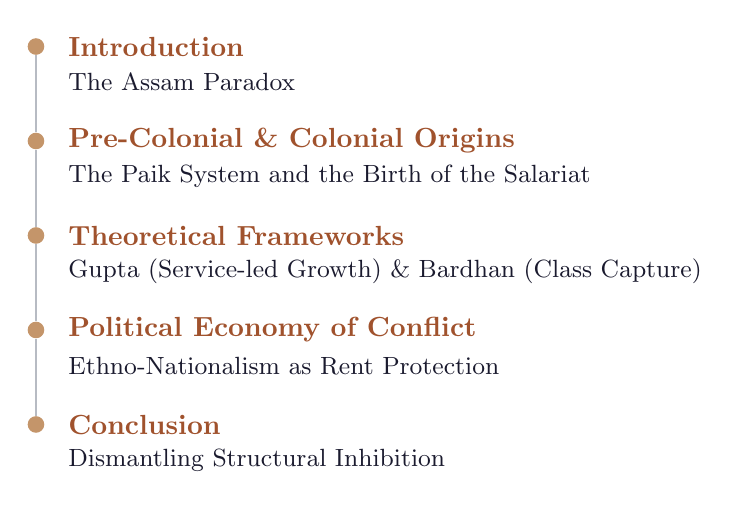
\begin{tikzpicture}[
    every node/.style={font=\normalsize, text=ink, anchor=west},
    sec/.style={font=\normalsize\bfseries, text=rust},
    dot/.style={circle, fill=clay, minimum size=6pt, inner sep=0pt},
    line/.style={slate!40, line width=0.8pt}
  ]
    \node[dot] (d1) at (0, 0) {};
    \node[sec] at (0.4, 0) {Introduction};
    \node[font=\small\color{slate}] at (0.4, -0.45) {The Assam Paradox};
    
    \node[dot] (d2) at (0, -1.2) {};
    \node[sec] at (0.4, -1.2) {Pre-Colonial \& Colonial Origins};
    \node[font=\small\color{slate}] at (0.4, -1.65) {The Paik System and the Birth of the Salariat};
    
    \node[dot] (d3) at (0, -2.4) {};
    \node[sec] at (0.4, -2.4) {Theoretical Frameworks};
    \node[font=\small\color{slate}] at (0.4, -2.85) {Gupta (Service-led Growth) \& Bardhan (Class Capture)};
    
    \node[dot] (d4) at (0, -3.6) {};
    \node[sec] at (0.4, -3.6) {Political Economy of Conflict};
    \node[font=\small\color{slate}] at (0.4, -4.05) {Ethno-Nationalism as Rent Protection};
    
    \node[dot] (d5) at (0, -4.8) {};
    \node[sec] at (0.4, -4.8) {Conclusion};
    \node[font=\small\color{slate}] at (0.4, -5.25) {Dismantling Structural Inhibition};
    
    % Connecting line
    \draw[line] (d1.south) -- (d2.north);
    \draw[line] (d2.south) -- (d3.north);
    \draw[line] (d3.south) -- (d4.north);
    \draw[line] (d4.south) -- (d5.north);
  \end{tikzpicture}
\end{minipage}
\end{frame}

\begin{frame}
\slidetitle{Where is Assam?}

\begin{center}
\vspace{-0.5cm}
\includegraphics[width=0.6\textwidth]{images/assam_map.jpg}
\vspace{-0.5cm}
\end{center}

{\small
\begin{center}
\begin{tabular}{lccc}
\toprule
\textbf{Indicator} & \textbf{Assam} & \textbf{India Avg} & \textbf{State Rank} \\
\midrule
Area (1000 km$^2$) & 78.4 & -- & 17th / 28 \\
Population 2021 (M) & 31.2 & -- & 15th / 28 \\
Per Capita Income (Rs) & 107k & 159k & \textcolor{burgundy}{\textbf{23rd / 28}} \\
\bottomrule
\end{tabular}
\end{center}
}
\end{frame}

\begin{frame}
\slidetitle{Introduction: The Assam Paradox}

\begin{columns}[T]
\column{0.5\textwidth}
\textbf{\color{rust}The Historical Reversal}
\begin{itemize}
  \item \textbf{Post-Independence:} Per capita income above national average
  \item \textbf{Current State:} Deficit widened to 45\% by 1990s
\end{itemize}

\vspace{6pt}
\begin{small}
\textbf{\color{slate}Conventional Explanations:}
\begin{itemize}
  \item[\textcolor{slate}{\rule[0.4ex]{4pt}{0.8pt}}] Geography: landlocked, poor connectivity
  \item[\textcolor{slate}{\rule[0.4ex]{4pt}{0.8pt}}] Resource curse: tea monoculture
\end{itemize}
\end{small}

\column{0.45\textwidth}
\critiquebox{Structural Stagnation}{%
 Persistently low capital formation, sluggish industrialization, hypertrophied service sector unable to generate broad-based employment.
}
\end{columns}

\vspace{8pt}
\thesisbox{The Political Economy Thesis}{%
  Geography and resources cannot explain why Assam failed to develop an indigenous capitalist class or why the state became captured by rent-seeking salaried elites. Underdevelopment is the endogenous result of class hegemony—institutional arrangements created a state apparatus oriented toward patronage rather than productive investment.
}
\end{frame}

\begin{frame}
\slidetitle{The Path to Stagnation: A Historical Timeline}

\vspace{0.3cm}
\begin{center}
  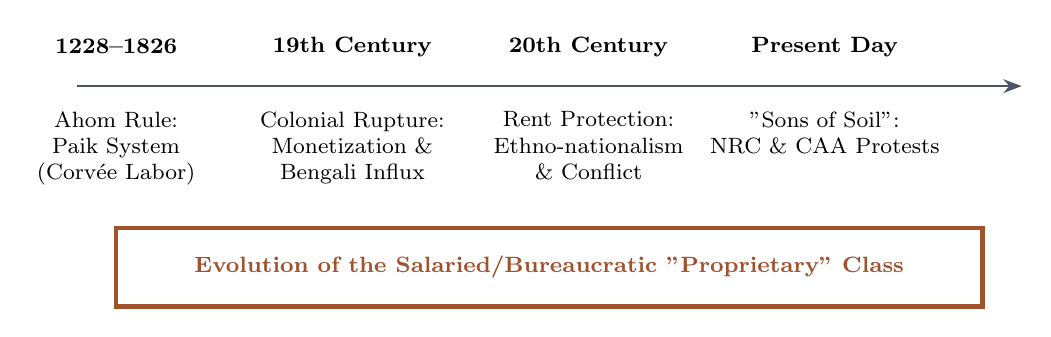
\begin{tikzpicture}[node distance=2cm, every node/.style={font=\footnotesize, align=center}]
    % Timeline Line
    \draw[thick, slate, -{Stealth}] (0,0) -- (12,0);
    
    % Nodes
    \node (n1) at (0.5, 0.5) {\textbf{1228--1826}};
    \node (n2) at (3.5, 0.5) {\textbf{19th Century}};
    \node (n3) at (6.5, 0.5) {\textbf{20th Century}};
    \node (n4) at (9.5, 0.5) {\textbf{Present Day}};

    \node[anchor=north] at (0.5, -0.2) {Ahom Rule: \\ Paik System \\ (Corv\'ee Labor)};
    \node[anchor=north] at (3.5, -0.2) {Colonial Rupture: \\ Monetization \& \\ Bengali Influx};
    \node[anchor=north] at (6.5, -0.2) {Rent Protection: \\ Ethno-nationalism \\ \& Conflict};
    \node[anchor=north] at (9.5, -0.2) {"Sons of Soil": \\ NRC \& CAA Protests};

    % Highlighting the "Service Class" Path
    \draw[rust, ultra thick] (0.5,-1.8) rectangle (11.5,-2.8);
    \node[rust] at (6,-2.3) {\textbf{Evolution of the Salaried/Bureaucratic "Proprietary" Class}};
  \end{tikzpicture}
\end{center}

\infobox{The Core Argument}{%
  Assam's economic trajectory was shaped by a historical path dependency that created an indigenous elite culturally averse to entrepreneurial risk, yet structurally incentivized to capture state resources through public sector employment.
}
\end{frame}

% ============================================================
\section{Introduction}
% ============================================================


% ============================================================
\section{Pre-Colonial Origins}
% ============================================================

\begin{frame}
\slidetitlesub{Precolonial Foundations}{The Ahom Paik System (1228-1826)}

\begin{columns}[T]
\column{0.55\textwidth}
\begin{itemize}
  \item \textbf{Corv\'ee Economy:} Non-monetized labor utilization mechanism. Every adult male (\textit{paik}) was obligated to render state service for cultivable land.
  \item \textbf{Egalitarian but Rigid:} No massive class of landless agricultural laborers existed (average peasant held 2.66 acres). The Neo-Vaishnavite movement thwarted rigid caste hierarchies.
  \item \textbf{Hereditary Administrative Hierarchy:} Key bureaucratic positions (Bora, Saikia, Phukan) were held by hereditary nobility. 
\end{itemize}

\column{0.4\textwidth}
\begin{center}
  \vspace{-6pt}
  \includegraphics[width=\linewidth,height=0.5\textheight,keepaspectratio]{images/guha_assam.jpg}
\end{center}
\end{columns}
\end{frame}

% === ADMINISTRATIVE HIERARCHY ===
\begin{frame}
\slidetitle{The Ahom Administrative Classes \& Paik Authority}

\begin{columns}[T]
\column{0.5\textwidth}
\textbf{\color{rust}Paik Officials \& Their Command}

\vspace{6pt}
\begin{center}
\small
\rowcolors{2}{cream}{parchment}
\begin{tabular}{@{}lc@{}}
\arrayrulecolor{warmgray}
\toprule
\textbf{Official} & \textbf{Paiks Commanded} \\
\midrule
\textbf{Phukan} & 6,000 \\
\textbf{Rajkhowa} & 3,000 \\
\textbf{Hazarika} & 1,000 \\
\textbf{Saikia} & 100 \\
\textbf{Bora} & 20 \\
\bottomrule
\end{tabular}
\end{center}

\vspace{6pt}
{\small\color{slate}These officials managed the corvée labor system reorganized in 1608.}

\column{0.45\textwidth}
\thesisbox{Merit vs. Heredity}{%
  Unlike later colonial bureaucracies (which emphasized merit through examinations), the Ahom state relied exclusively on \textbf{hereditary merit}. Administrative positions were family inheritances, not competitive positions accessible to educated commoners.
}

\vspace{8pt}
{\footnotesize\textit{\color{slate}Source: Sen, Debasis (1979). ``A Few Aspects of the Ahom Military System.'' \textit{Proceedings of the Indian History Congress}, 40: 552--556.}}
\end{columns}
\end{frame}

% === PAIK POPULATION TABLE ===
\begin{frame}
\slidetitle{Paik Population Estimates (c. 1711)}

\vspace{6pt}
\begin{center}
\small
\begin{tabular}{ccc}
\arrayrulecolor{warmgray}
\toprule
\textbf{Paiks (millions)} & \textbf{Male Population (millions)} & \textbf{Total Population (millions)} \\
\midrule
0.26 & 0.52 & 2.08 \\
0.36 & 0.72 & 2.88 \\
0.40 & 0.80 & 3.20 \\
\bottomrule
\end{tabular}
\end{center}

\vspace{10pt}
\begin{columns}[T]
\column{0.48\textwidth}
\infobox{The Militia State}{%
  King Rudra Singha's militia register revealed that 260,000--400,000 paiks could be mobilized for warfare, representing a massive state apparatus built on corvée labor.
}

\column{0.48\textwidth}
\critiquebox{Overwhelmingly Rural}{%
  The capital city Rangpur had only 10,000 inhabitants in 1794. Urban population was estimated at less than 2\% of the total---merchants and capitalists were virtually absent.
}
\end{columns}
\end{frame}

% === BENGAL-AHOM TRADE TABLE ===
\begin{frame}
\slidetitle{Pre-Colonial Trade: Bengal-Ahom Exchange}

\vspace{4pt}
\begin{center}
\tiny
\begin{tabular}{lrc|lrc}
\arrayrulecolor{warmgray}
\toprule
\multicolumn{3}{c|}{\textbf{\color{rust}Exports from Bengal}} & \multicolumn{3}{c}{\textbf{\color{deepgreen}Imports from Assam}} \\
\textbf{Good} & \textbf{Quantity} & \textbf{Value} & \textbf{Good} & \textbf{Quantity} & \textbf{Value} \\
\midrule
Salt & 35 & 192.5 & Stick-lac & 10 & 35.0 \\
Ghi & 1 & 1.6 & Raw Cotton & 7 & 35.0 \\
Fine pulses & --- & 0.8 & Muga Silk & 0.1 & 28.9 \\
Sugar, Spices & --- & 2.0 & Mustard & 15 & 20.0 \\
Copper & --- & 4.8 & Ivory & --- & 6.5 \\
Red bead, paints & --- & 1.5 & Bell-metal vessels & --- & 2.1 \\
Stone beads & --- & 8.0 & Black Pepper & 0.1 & 0.8 \\
European glassware & --- & 2.5 & Indian madder & --- & 0.5 \\
Muslin & --- & 10.0 & Thaikal & --- & 0.1 \\
Other luxury & --- & 4.5 & Slaves & --- & 2.0 \\
\midrule
\multicolumn{2}{l}{\textbf{Subtotal}} & \textbf{228.2} & \multicolumn{2}{l}{\textbf{Subtotal}} & \textbf{130.9} \\
Cowries & 0.1 & --- & Gold \& Silver & --- & \textbf{\color{burgundy}97.4} \\
\midrule
\multicolumn{2}{l}{\textbf{Total}} & \textbf{228.3} & \multicolumn{2}{l}{\textbf{Total}} & \textbf{228.3} \\
\bottomrule
\multicolumn{6}{l}{\tiny\textit{Source: Hamilton (1940), Anglo-Assamese Relations. Values in thousands of rupees.}} \\
\end{tabular}
\end{center}

\vspace{8pt}
\thesisbox{No Merchant Class?}{%
  Assam ran a persistent trade deficit of 97,400 rupees, paid exclusively in gold and silver bullion. Unlike Gujarat (which had Rs. 16 million in trade via Surat), Assam had minimal global trade presence and virtually no merchant class to develop indigenous capitalism.
}
\end{frame}

\section{Colonial Rupture}
\begin{frame}
\slidetitlesub{Colonial Rupture}{Monetization and Linguistic Displacement}

\begin{columns}[T]
\column{0.48\textwidth}
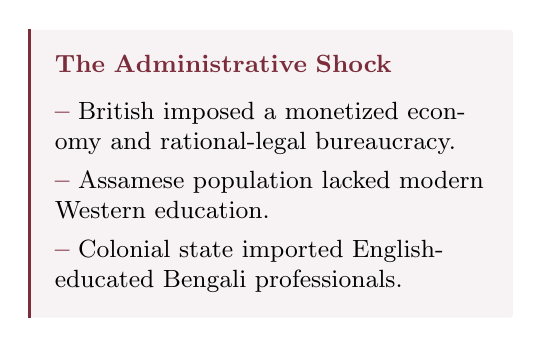
\begin{tikzpicture}
  \node[
    fill=burgundy!6, inner sep=9pt, text width=5.5cm,
    rounded corners=1pt, font=\small
  ] (z) {%
    {\bfseries\color{burgundy}The Administrative Shock}\\[6pt]
    {\color{burgundy}\textbf{--}} British imposed a monetized economy and rational-legal bureaucracy.\\[3pt]
    {\color{burgundy}\textbf{--}} Assamese population lacked modern Western education.\\[3pt]
    {\color{burgundy}\textbf{--}} Colonial state imported English-educated Bengali professionals.
  };
  \draw[burgundy, line width=1.2pt] (z.north west) -- (z.south west);
\end{tikzpicture}

\column{0.48\textwidth}
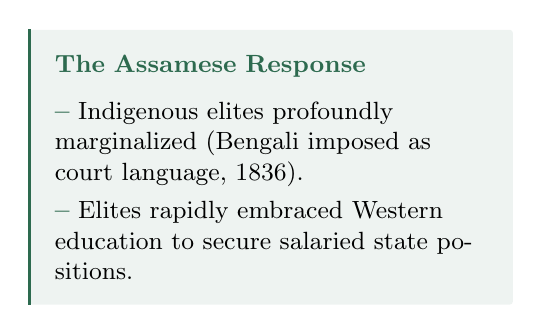
\begin{tikzpicture}
  \node[
    fill=deepgreen!8, inner sep=9pt, text width=5.5cm,
    rounded corners=1pt, font=\small
  ] (r) {%
    {\bfseries\color{deepgreen}The Assamese Response}\\[6pt]
    {\color{deepgreen}\textbf{--}} Indigenous elites profoundly marginalized (Bengali imposed as court language, 1836).\\[3pt]
    {\color{deepgreen}\textbf{--}} Elites rapidly embraced Western education to secure salaried state positions.
  };
  \draw[deepgreen, line width=1.2pt] (r.north west) -- (r.south west);
\end{tikzpicture}
\end{columns}

\vspace{10pt}
\critiquebox{A State-Dependent Class}{%
  Unlike mercantile capitalists in western India, the Assamese middle class did not rise through mercantile trade or industrial innovation. Their prestige and security were directly tied to colonial state proximity and government salaries.
}
\end{frame}

\section{Theoretical Frameworks}
% ============================================================

\begin{frame}
\slidetitlesub{Theoretical Framework I}{Bishnupriya Gupta: Educational Bias \& Service-Led Growth}

\begin{columns}[T]
\column{0.48\textwidth}
{\bfseries\color{ink}The Historical Roots of Services}
\begin{itemize}
  \item Challenges the assumption that service-led growth was triggered by 1990s economic liberalization; it possesses deep historical roots.
  \item \textbf{Productivity Divergence:} Between 1870 and 1970, Indian agriculture plummeted, but comparative labor productivity in the service sector consistently rose from 15\% to 30\% of the UK level.
\end{itemize}

\column{0.48\textwidth}
{\bfseries\color{ink}The Colonial Education Matrix}
\begin{itemize}
  \item The colonial state underinvested in mass primary education, which is the foundational prerequisite for an industrial or agricultural transition.
  \item Instead, education was heavily biased toward secondary and tertiary levels, catering exclusively to elites desiring rent-yielding administrative positions.
\end{itemize}
\end{columns}
\end{frame}

% ============================================================

\begin{frame}
\slidetitlesub{The Assamese Manifestation}{Educational Credentials for Rent Extraction}

\begin{small}
\begin{center}
\begin{tabular}{lc}
\toprule
\textbf{Province/Region} & \textbf{Literate in English (Per 10,000 Males)} \\
\midrule
\textbf{Assam} & \textbf{87} \\
Bombay & 60 \\
Mysore & 51 \\
Madras & 44 \\
Bengal & 35 \\
Central Provinces & 18 \\
\bottomrule
\multicolumn{2}{l}{\small\textit{Source: Gupta (2025).}} \\
\end{tabular}
\end{center}
\end{small}

\vspace{11pt}
\thesisbox{The Educational Paradox in Assam}{%
  Assam produced a highly educated elite whose skill sets were exclusively tailored for the tertiary service sector. Because they culturally eschewed commerce, their human capital was never deployed to create manufacturing firms or logistics networks. Instead, education was deployed strictly as a credential to extract salaries from the state.
}
\end{frame}

% ============================================================

\begin{frame}
\slidetitlesub{Theoretical Framework II}{Pranab Bardhan: Dominant Proprietary Classes (1984)}

\begin{columns}[T]
\column{0.47\textwidth}
\begin{tikzpicture}
  \node[
    fill=ochre!10, inner sep=10pt, text width=5.3cm,
    rounded corners=2pt, font=\small
  ] (w1) {%
    {\color{ochre}\faUniversity}\quad{\bfseries\color{ink}The Rent-Seeking Coalition}\\[6pt]
    Bardhan argues Indian state policy is dictated by a frequently conflicting coalition of three "dominant proprietary classes":\\[4pt]
    \textbullet\ Industrial Capitalists\\
    \textbullet\ Rich Farmers\\
    \textbullet\ \textbf{Public Sector Professionals}\\[6pt]
    Educational credentials and permanent government positions function precisely as a form of property that yields continuous economic rents.
  };
  \draw[ochre, line width=1.5pt] (w1.north west) -- (w1.south west);
\end{tikzpicture}

\column{0.47\textwidth}
\begin{tikzpicture}
  \node[
    fill=deepgreen!8, inner sep=10pt, text width=5.3cm,
    rounded corners=2pt, font=\small
  ] (w2) {%
    {\color{deepgreen}\faBan}\quad{\bfseries\color{ink}The Collective Action Problem}\\[6pt]
    This elite coalition exerts immense pressure on the state to distribute patronage and allocate subsidies.\\[6pt]
    \textbf{Result:} The state becomes paralyzed. It cannot pursue long-term, capital-accumulating macroeconomic policies because its fiscal resources are constantly drained to satisfy immediate rent-seeking demands.
  };
  \draw[deepgreen, line width=1.5pt] (w2.north west) -- (w2.south west);
\end{tikzpicture}
\end{columns}
\end{frame}

% ============================================================

\begin{frame}
\slidetitlesub{The Monopoly of the Salariat}{Applying Bardhan to Assam}

\begin{columns}[T]
\column{0.5\textwidth}
\textbf{\color{rust}The Missing Classes}
\begin{itemize}
  \item \textbf{No Capitalists:} The Assamese failed to develop an industrial class. Commerce was left to immigrants who possessed wealth but lacked indigenous political legitimacy to dictate state policy openly.
  \item \textbf{No Powerful Landlords:} The British Ryotwari system prevented the emergence of a politically powerful class of landed gentry or absentee landlords.
\end{itemize}

\column{0.45\textwidth}
\infobox{Unrivaled Hegemony}{%
  With both capitalists and rich farmers absent, the third leg of Bardhan's triad—the professional salaried class—achieved an unrivaled, monopolistic hegemony over Assam's political economy. 
}
\end{columns}

\vspace{10pt}
\centering
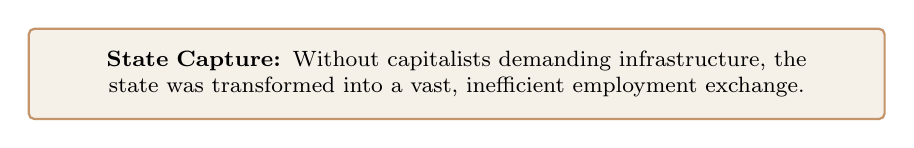
\begin{tikzpicture}
  \node[
    draw=clay, line width=0.8pt, rounded corners=2pt,
    fill=cream, inner sep=8pt, font=\footnotesize,
    text width=0.85\textwidth, align=center
  ] {%
    \textbf{State Capture:} Without capitalists demanding infrastructure, the state was transformed into a vast, inefficient employment exchange.
  };
\end{tikzpicture}
\end{frame}

% ============================================================
\section{Political Economy of Conflict}
% ============================================================

\begin{frame}
\slidetitle{Ethno-Nationalism as Rent Protection}

\begin{columns}[T]
\column{0.47\textwidth}
\critiquebox{Vulnerability of the Salariat}{%
  The Assamese salariat had no private industrial base or mercantile networks. Any perceived demographic threat to their monopoly over government jobs was viewed as a literal existential crisis.
}

\vspace{6pt}
\begin{itemize}
  \item \textbf{Identity Politics:} The salariat mobilized sub-nationalist movements (language agitations, the Assam Movement) to carve out protected administrative territories guaranteeing preferential treatment in public employment.
\end{itemize}

\column{0.47\textwidth}
\vspace{2pt}
\infobox{Behavioral Economics of Conflict}{%
  \begin{itemize}
    \item[{\color{deepgreen}\rule[0.4ex]{4pt}{0.8pt}}] Exposure to extreme violence fundamentally alters attitudes toward risk-taking and reduces cooperative behavior.
    \item[{\color{deepgreen}\rule[0.4ex]{4pt}{0.8pt}}] Strikes and systemic extortion drive away private investment.
    \item[{\color{deepgreen}\rule[0.4ex]{4pt}{0.8pt}}] Without private sector growth, youth are forced to double down on demands for government jobs.
  \end{itemize}%
}
\end{columns}
\end{frame}

% ============================================================
\section{Conclusion}
% ============================================================

\begin{frame}
\slidetitle{Conclusion}

\vspace{10pt}
\begin{itemize}
  \item[\textcolor{rust}{\textbf{1.}}] \textbf{Path Dependency:} Assam's pre-colonial Paik system created a cultural affinity for state patronage.
  
  \vspace{8pt}
  \item[\textcolor{rust}{\textbf{2.}}] \textbf{Class Hegemony:} Without capitalists or powerful landlords, the professional salariat achieved monopolistic control over the state apparatus.
  
  \vspace{8pt}
  \item[\textcolor{rust}{\textbf{3.}}] \textbf{Post Colonial:} Segments of the middle class unable to access stable employment grew increasingly dissatisfied, pressing the state for quotas through anti-migrant ``sons-of-soil'' movements (Fernandes 2006). In Assam, from the 1950s--1970s, middle class movements centered explicitly on job scarcity, reinforcing the structural dependence on state patronage. 
  \vspace{8pt}
  \item[\textcolor{rust}{\textbf{3.}}] \textbf{As Things Stand:} NRC \& CAA Protests 
\end{itemize}
\end{frame}

% ============================================================
% CLOSING SLIDE
% ============================================================

\begin{frame}[plain]
\begin{tikzpicture}[remember picture, overlay]
  % Background
  \fill[parchment] (current page.south west) rectangle (current page.north east);
\end{tikzpicture}

\vspace{1.5cm}
\begin{columns}[c]
\column{0.65\textwidth}
\hspace{60pt}\begin{minipage}{0.85\textwidth}
  {\fontsize{32}{36}\selectfont\color{ink}\textbf{Thank You}}
  
  \vspace{8pt}
  {\color{ochre}\rule{50pt}{3pt}}
  
  \vspace{16pt}
  {\fontsize{16}{20}\selectfont\color{ink}\bfseries Questions \& Discussion}
  
  \vspace{20pt}
  {\Large\color{ink}\textbf{Kabeer Bora}}\\[4pt]
  {\large\color{ink}University of Missouri--Kansas City}\\[4pt]
  
  \vspace{16pt}
  {\normalsize\color{ink}\textit{Suggestions/Feedback Welcome!}}\\[2pt]
  {\small\color{ink}\textit{Email: \href{kabeerbora@umkc.edu}{kabeerbora@umkc.edu}}}
\end{minipage}

\column{0.3\textwidth}
\centering
\vspace{-1cm}

\begin{tikzpicture}
  \node[fill=white, inner sep=8pt, rounded corners=3pt] {
    \qrcode[height=3.5cm]{https://github.com/kabeerbora/assam-presentation/raw/main/presentation.pdf}
  };
\end{tikzpicture}

\vspace{17pt}

{\small\color{ink}\textbf{Download Slides}}
\end{columns}
\end{frame}

\end{document}
